% !TEX encoding = UTF-8 Unicode
% -*- coding: UTF-8; -*-
% vim: set fenc=utf-8
\documentclass[a4paper,12pt,fleqn]{article}
\usepackage[a4paper, total={6.5in, 9in}]{geometry}

\usepackage{multirow}
\usepackage{comment}
\usepackage[table,xcdraw]{xcolor}
\usepackage{centrale}
\usepackage{minted}
\usepackage{enumitem}
\usepackage[thinlines]{easytable}
\usepackage{tikz}
\usetikzlibrary{graphdrawing.trees}
\usegdlibrary{trees}

\usepackage{graphicx}       % provides commands for including figures
\usepackage{csquotes}       % provides \enquote{} macro for "quotes"
\usepackage{glossaries}     % provides glossary commands

\usetikzlibrary{matrix,backgrounds}

\newcommand\ezskip{\medskip\noindent}

\lstset{
    frame=tb, % draw a frame at the top and bottom of the code block
    tabsize=4, % tab space width
    showstringspaces=false, % don't mark spaces in strings
    numbers=left, % display line numbers on the left
    commentstyle=\color{green}, % comment color
    keywordstyle=\color{blue}, % keyword color
    stringstyle=\color{red} % string color
}

\hypersetup{
    pdftitle={APP2 Report},
    pdfauthor={Eslam Mohammed, Habib Slim, Albert Strümpler, Sofiane Tanji, Manuel Treutlein, Archit Yadav},
    pdfsubject={Problem Solving},
    pdfproducer={},
    pdfkeywords={greedy, dynamic programming, complete solution space exploration, holdem, cards} %
}

\DeclareGraphicsRule{.ai}{pdf}{.ai}{} % pour insérer des documents .ai
\graphicspath{ {./img/} {./eps/}} % pour ne pas avoir à ajouter eps/ton-image.jpg

% ------------- Packages spéciaux, nécessaires pour ce rapport, à insérer ici ------------- 

\begin{document}

% --------------------------------------------------------------
%                       Page de garde
% --------------------------------------------------------------

\begin{titlepage}
\begin{center}


\includegraphics[width=0.35\textwidth]{logo-uga.png}
\includegraphics[width=0.35\textwidth]{logoinp.png} \\[1cm]

{\large Master M1 MOSIG – UGA \& Grenoble INP} \\[0.8cm]
{\large Algorithmic Problem Solving}\\[0.5cm]

% Title
\rule{\linewidth}{0.5mm} \\[0.4cm]
{ \huge \bfseries APP2: Hold’em for n00bs \\[0.4cm] }
\rule{\linewidth}{0.5mm} \\[1.5cm]

% Author and supervisor
\noindent
\begin{minipage}{0.4\textwidth}
  \begin{flushleft} \large
    \emph{Authors :}\\
    Eslam \textsc{Mohammed}\\
    Habib \textsc{Slim}\\
    Albert \textsc{Strümpler}\\
    Sofiane \textsc{Tanji}\\
    Manuel \textsc{Treutlein}\\
    Archit \textsc{Yadav}
  \end{flushleft}
\end{minipage}%
\begin{minipage}{0.4\textwidth}
  \begin{flushright} \large
    \emph{Teacher :} \\
    Ms.~Malin \textsc{Rau}\\
  \end{flushright}
\end{minipage}

\vfill

% Bottom of the page
{\large Last Version \\ \today}

\end{center}
\end{titlepage}

% --------------------------------------------------------------
%                    Table des matières 
% --------------------------------------------------------------

\thispagestyle{empty}
\tableofcontents
\newpage
% --------------------------------------------------------------
%                         Début du corps
% --------------------------------------------------------------
\section{Introduction} \label{sec:introduction}
% Explanation of the problem and modelling.
In this APP we have to deal with a card game played by two persons.
A sequence of n cards lying on a table face up in a line. The two players take turns choosing a card from the leftmost or rightmost end. It is not allowed to take a card which is not at one of the two ends. After one player takes the last card, the game is over. The player with the higher card sum in the end wins. The figure \ref{fig:introductionExample} shows an example of a possible card game.

\begin{figure}[H]
    \centering
    \begin{tikzpicture}[font=\ttfamily,
    array/.style={matrix of nodes,nodes={draw, minimum size=7mm},column sep=-\pgflinewidth, row sep=0mm, nodes in empty cells,
    row 1/.style={nodes={draw=none, fill=none, minimum size=5mm}},
    row 1 column 1/.style={nodes={draw}},
    row 1 column 10/.style={nodes={draw}}}]
    
    \matrix[array] (array) {
    4 & 3 & 5 & 2 & 2 & 14 & 13 & 5 & 7 & 9\\};
    
    \end{tikzpicture}
    \caption{Example of a card game. Card 4 and 9 can be chosen from the current player.}
    \label{fig:introductionExample}
\end{figure}

In this APP we decided to change to python code for representing algorithms.
The reason for this is that python code has a simple structure and resembles to
pseudo-code in a way. Additionally, it allows us to represent the developed
algorithms in a more detailed way.

\ezskip One player, named the sister, will always play the so called greedy strategy. Therefore we first consider an algorithm applying this method in chapter \ref{sec:greedySol}. Because of some limitations of the greedy strategy we will then consider a complete solution space exploration in chapter \ref{sec:completeSol}. This gives us an optimal solution, but with an unacceptable runtime. For this reason we will introduce a dynamic algorithm in chapter \ref{sec:dp_solution}, resulting in an optimal solution with acceptable runtime. Before we begin with the algorithms, we will introduce in chapter \ref{sec:notations} some notations. 

\newpage
\section{Notations} \label{sec:notations}

In the following, one player is referred to as the sister, the other player is referred to as the strategist.

For all of what follows, we will be using the same data structure to represent the playing cards : a simple array of fixed size containing all card costs that have been drawn, unordered, named "\texttt{CARDS}". The elements of \texttt{CARDS} are $integers$ in the range of $[2, 14]$, whereas the value $2$ represents the card two and the value $14$ represents the value of an ace. All values in between are assigned appropriately, this means in particular for the face cards that the jack is modeled by $11$, the queen by $12$ and the king by $13$.

%% TODO change this section if input or output should be different
The input of all algorithms is a list of cards represented as array \texttt{CARDS} and the choice of the sister about who makes the first move, represented as a $boolean$.

In order to visually describe a configuration of cards in a game, we will be using the following diagram notations :

\begin{figure}[H]
    \centering
    \begin{tikzpicture}[font=\ttfamily,
    array/.style={matrix of nodes,nodes={draw, minimum size=7mm},column sep=-\pgflinewidth, row sep=0mm, nodes in empty cells,
    row 1/.style={nodes={draw=none, fill=none, minimum size=5mm}},
    row 1 column 1/.style={nodes={draw}},
    row 1 column 10/.style={nodes={draw}}}]
    
    \matrix[array] (array) {
    0 & 1 & 2 & 3 & 4 & 5 & 6 & 7 & 8 & 9\\
    3 & 2 & 7 & 8 & 9 & 10&14 & 6 & 4 & 3\\};
    
    \begin{scope}[on background layer]
    \fill[CentraleRed!20] (array-1-1.north west) rectangle (array-1-10.south east);
    \end{scope}
    
    \draw (array-1-1.north)--++(90:3mm) node [above] (first) {\textbf{i}};
    \draw (array-1-10.north)--++(90:3mm) node [above] (first) {\textbf{j}};
    \draw (array-1-10.east)--++(0:3mm) node [right]{Indices};
    \draw (array-2-10.east)--++(0:3mm) node [right]{Card costs};
    %
    \end{tikzpicture}
    \caption{Initial configuration}
    \label{fig:example_diag_01}
\end{figure}

More generally, a configuration $(i,j)$ describing a situation produced from a set of $n$ cards is such that:

$$ (i,j) \in [\![0,\ n-1]\!]^2, \ i \leq j $$

If $i$ is equal to $j$, we are describing a configuration in which a single card of index $i$ ($= j$) and of cost \texttt{CARDS[i]} (\texttt{= CARDS[j]}) is remaining.

\medskip

Referring to the subconfiguration $(i+1,\ j)$ thus describes a subsequent configuration in which the first player picked the left-most card (here, of cost 3), like shown in figure \ref{fig:example_diag_02}.

\begin{figure}[H]
    \centering
    \begin{tikzpicture}[font=\ttfamily,
    array/.style={matrix of nodes,nodes={draw, minimum size=7mm},column sep=-\pgflinewidth, row sep=0mm, nodes in empty cells,
    row 1/.style={nodes={draw=none, fill=none, minimum size=5mm}},
    row 1 column 2/.style={nodes={draw}},
    row 1 column 10/.style={nodes={draw}}}]
    
    \matrix[array] (array) {
    0 & 1 & 2 & 3 & 4 & 5 & 6 & 7 & 8 & 9\\
    3 & 2 & 7 & 8 & 9 & 10&14 & 6 & 4 & 3\\};
    
    \begin{scope}[on background layer]
    \fill[CentraleRed!20] (array-1-1.north west) rectangle (array-1-10.south east);
    \fill[gray!80] (array-2-1.north west) rectangle (array-2-1.south east);
    \end{scope}
    
    \draw (array-1-2.north)--++(90:3mm) node [above] (first) {\textbf{i+1}};
    \draw (array-1-10.north)--++(90:3mm) node [above] (first) {\textbf{j}};
    %
    \end{tikzpicture}
    \caption{Following subconfiguration}
    \label{fig:example_diag_02}
\end{figure}

The card of index 0 and of cost 3 has been greyed out, which means that it was selected and can no longer be picked and added to a player's score.

\medskip

In general, referring to the subconfiguration $(i+n,\ j-k)$ describes a configuration in which $n$ cards have been picked on the left-side of the stack, and $k$ cards have been picked on the right side. Obviously, the constraint $i+n \leq j-k$ must be correct for the configuration to be valid.

% --------------------------------------------------------------
%                         Part 1
% --------------------------------------------------------------

\newpage

\section{The greedy algorithm} \label{sec:greedySol}
As presented in the introduction, the first algorithm we studied was the greedy algorithm, it is the method that the sister always uses when she plays the game. In the first part, the strategist player also plays greedy to understand the concept and also to see the algorithm evolution through this APP development.

\ezskip The greedy algorithm consists in choosing the local optimal choice at each step. It is a naive approach that is preferring what looks like the better choice but may not be globally because of the missing information that isn't considered. In our case the algorithm always picks the biggest card from the two possibilities without considering the other cards.

\ezskip The tree in figure \ref{fig:greedy_01} shows the possibilities for a greedy player trying to pick the best score out of the card deck against another greedy player notated $">"$. As we can see the greedy player always picks the biggest card, but didn't get the best possible result at the end and didn't win.

\begin{figure}[H]
    \centering   
    \begin{tikzpicture}[font=\ttfamily,
    array/.style={matrix of nodes,nodes={draw, minimum size=7mm},column sep=-\pgflinewidth, row sep=0mm, nodes in empty cells,
    row 1/.style={nodes={draw=none, fill=none, minimum size=5mm}}}]

    \matrix[array] (array) {
    0 & 1 & 2 & 3 & 4 & 5\\
    14& 13& 5 &12 & 2 & 4\\};

    \begin{scope}[on background layer]
    \fill[CentraleRed!20] (array-1-1.north west) rectangle (array-1-6.south east);
    \end{scope}
    \end{tikzpicture}

    \begin{tikzpicture}[nodes={draw, circle}, ->]
        \node {Start}
        child { node [fill=CentraleRed!60] {14 \tiny{>13}} 
            child{ node [fill=CentraleRed!60] {5 \tiny{>12}} 
                child{ node [fill=CentraleRed!60] {4  \tiny{>2}}}
                child{ node {2 \tiny{>4}}}
            }
            child [missing]
            child{ node [fill=yellow!50!red] {4 \tiny{>5}} 
                child{node [fill=yellow!50!red] {12 \tiny{>2}}}
                child{node {2 \tiny{>12}}}
            }
        }
        child [missing]
        child [missing]
        child [missing]
        child { node [fill=yellow] {4 \tiny{>14}} 
            child{ node [fill=yellow] {13 \tiny{>5}} 
                child{node [fill=yellow] {12 \tiny{>2}}}
                child{node {2 \tiny{>12}}}
            }
            child [missing]
            child{ node {2 \tiny{>13}} 
                child{node {12 \tiny{>5}}}
                child{node {5 \tiny{>12}}}
            }
        };
    \end{tikzpicture}
    \caption{Greedy Choices (green), Best Solution (orange), Better than greedy (yellow)}
    \label{fig:greedy_01}
\end{figure}

\newpage

\subsection{Pseudocode}
Depending on whether the sister starts or not (meaning if the boolean \texttt{sisterFirst} is equal to \texttt{True} or \texttt{False}), \texttt{getScores} computes the resulting scores of the player and the sister when both are playing greedy.
\begin{minted}[frame=leftline]{Python}
def getScores(sisterFirst):
    sum_sister, my_sum = 0, 0
    i, j = 0, len(CARDS) - 1
    if sisterFirst:
        while i <= j:
            # Sister's turn
            if CARDS[i] > CARDS[j]:
                sum_sister += CARDS[i]
                i += 1
            else:
                sum_sister += CARDS[j]
                j -= 1
            # Brother's turn
            if CARDS[i] > CARDS[j]:
                my_sum += CARDS[i]
                i += 1
            else:
                my_sum += CARDS[j]
                j -= 1
    else:
        while i <= j:
            # Brother's turn
            if CARDS[i] > CARDS[j]:
                my_sum += CARDS[i]
                i += 1
            else:
                my_sum += CARDS[j]
                j -= 1

            # Sister's turn
            if CARDS[i] > CARDS[j]:
                sum_sister += CARDS[i]
                i += 1
            else:
                sum_sister += CARDS[j]
                j -= 1
    return my_sum, sum_sister
\end{minted}

\subsection{Complexity, limitations and advantages}
%% TODO complete, RESPONSIBLE PERSON: Manuel
Most greedy algorithms have several characteristics in common. 
Our greedy algorithm for solving the considered problem is no exception. 
As a quick overview, consider the table \ref{tab:greedyAdLi}. 
\begin{table}[H]
    \centering
    \begin{tabular}{c|c}
        \textbf{Advantages} & \textbf{Limitations} \\
        good runtime & not optimal \\
        no extra space & \\
        quick to implement & \\
        easy to understand & \\
    \end{tabular}
    \caption{Advantages and limitations of the greedy algorithm}
    \label{tab:greedyAdLi}
\end{table}{}

As shown in table \ref{tab:greedyAdLi}, the list of advantages of a greedy approach is quite appealing. The most important reason for using greedy algorithms is the good run time. Because a greedy algorithm decides locally and without adaptation later on, decisions are made fast. In our case this means a greater or smaller comparison between two integer values for one decision step. The decision is made for all $n$ cards. Because the comparison is a constant operation, we can conclude that the greedy algorithm is in $O(n)$. The worst and best case do not differ and are therefore in $O(n)$ as well. 

\ezskip Another advantage is that we do not have to store anything, except of the array \texttt{CARDS} itself. The implementation is done very quickly, in particular we do not need any special data structures or complex algorithms. The idea of the algorithm is intuitively and therefore easy to understand.\\
So why isn't it possible to stick to this smart solution? The answer is the non optimal solution finding in the global context. Optimal local decisions don't necessarily lead to optimal global solutions. Furthermore, we can think of examples where the greedy algorithm leads into something we could consider a dead end. 
% TODO dead end example 

For this reason we have to look at different approaches in the following chapters. 

% --------------------------------------------------------------
%                         Part 2
% --------------------------------------------------------------

\newpage

\section{Complete solution space exploration} \label{sec:completeSol}
%% TODO complete, RESPONSIBLE PERSON: Albert
The aim of the complete solution space exploration is to find every
possible solution for our problem. Therefore we ensure that we find
an optimal solution for our problem. 

You can compare our solution in the following pseudocode with the figure \ref{fig:CSS_01}. We have to find every possible branch for the solution. Don't forget that this may not be the solution of the greedy algorithm as seen in figure \ref{fig:greedy_01}. 


\begin{figure}[H]
    \centering   
    \begin{tikzpicture}[font=\ttfamily,
    array/.style={matrix of nodes,nodes={draw, minimum size=7mm},column sep=-\pgflinewidth, row sep=0mm, nodes in empty cells,
    row 1/.style={nodes={draw=none, fill=none, minimum size=5mm}}}]

    \matrix[array] (array) {
    0 & 1 & 2 & 3 & 4 & 5\\
    14& 6 & 9 & 2 & 12& 3\\};

    \begin{scope}[on background layer]
    \fill[CentraleRed!20] (array-1-1.north west) rectangle (array-1-6.south east);
    \end{scope}
    \end{tikzpicture}


    \begin{tikzpicture}[nodes={draw, circle}, ->]
        \node {Start}
        child { node [fill=CentraleRed!60] {14 \tiny{>6}} 
            child{ node [fill=CentraleRed!60] {9 \tiny{>3}} 
                child{ node {2  \tiny{>12}}}
                child{ node [fill=CentraleRed!60] {12 \tiny{>2}}}
            }
            child [missing]
            child{ node {3 \tiny{>12}} 
                child{node {9 \tiny{>2}}}
                child{node {2 \tiny{>9}}}
            }
        }
        child [missing]
        child [missing]
        child [missing]
        child { node {3 \tiny{>14}} 
            child{ node {6 \tiny{>12}} 
                child{node {9 \tiny{>2}}}
                child{node {2 \tiny{>9}}}
            }
            child [missing]
            child{ node {12 \tiny{>6}} 
                child{node {9 \tiny{>2}}}
                child{node {2 \tiny{>9}}}
            }
        };
    \end{tikzpicture}
    \caption{Strategist's best solution (Index values are the sister's picks)}
    \label{fig:CSS_01}
\end{figure}

\newpage

\subsection{Pseudocode}
%% TODO complete, RESPONSIBLE PERSON: Habib, Jimmy
We explained that for doing the complete solution space exploration we have to find all possible branches in the corresponding tree. This leads to an algorithm draft where we construct this tree and compute the sum of all branches. Logically, the branch with the highest sum represents the best solution. Nonetheless we decided to use another version in which we don't have to store the whole tree, but compare the best solution 'on the fly'. For this purpose we define a binary number which represents a possible solution strategy for the cards game.

\ezskip The strategist player has to do $LEN\_CARDS/2$ number of choices. Therefore the number for the solution strategy consists of $LEN\_CARDS/2$ bits. A bit 0 indicates to take the leftmost card, a 1 indicates to take the rightmost card. The strategy is 'incremented' with 1 for every while loop, which means that all the strategies are tested one after another. We stop if we reached the strategy only containing ones. The pseudocode is separated in two functions. The application of the current solution strategy is outsourced.

\ezskip The \texttt{applySolution} function returns the sum for the strategist with regards to the \texttt{solutionStrategy}. We update the best value respectively the best strategy if the return of a new \texttt{solutionStrategy} is better than our current best solution. After we finished going through all possible solutions we can return the best solution. 

\begin{minted}[frame=leftline]{Python}
def completeSolutionSpaceExploration(CARDS, sisterFirst):
    # Define the solutionStrategy in a binary format.
    # If the value is 0, the player should choose the leftmost
    # card, 1 for the rightmost card.
    solutionStrategy = 0b0
    # We reach the last solutionStrategy if the solutionStrategy
    # only consists of one. For a player are LEN_CARDS/2 choices
    # in one game because there are two players for LEN_CARDS number
    # of cards. This leads to exponential choices. With bin() we convert
    # the decimal value into a binary.
    if sisterFirst 
        numberOfChoices = floor(LEN_CARDS / 2)
    else 
        numberOfChoices = ceil(LEN_CARDS / 2)
    lastSolutionStrategy = bin(pow(2, numberOfChoices))

    # Store the best solutions here.
    bestSolutionValue = 0
    bestSolutionStrategy = 0b0

    while solutionStrategy is not lastSolutionStrategy :
        newSolutionValue = applySolution(sisterFirst, solutionStrategy)
        if newSolutionValue > bestSolutionValue :
            bestSolutionValue = newSolutionValue
            bestSolutionStrategy = solutionStrategy
        solutionStrategy++

    return (bestSolutionStrategy, bestSolutionValue)

def applySolution(sisterFirst, solutionStrategy)
    # Save the current round. One round is one card choice
    # of the sister and one of the strategist.
    currentRound = 1
    # sum up the result for the strategist.
    sum = 0
    i = 0
    j = LEN_CARDS - 1

    while i != j
        if (sisterFirst):
            # Sister takes the local optimum
            if (CARDS[i] > CARDS[j]):
                i++
            else:
                j -= 1
        else:
            # Here we apply the solutionStrategy, the strategist
            # follows the solutionStrategy.
            # We choose the card depending on the bit in the 
            # solution strategy. We get the correct bit with 
            # the bitAtPos() function with the informal signature:
            # bitAtPos() : position --> binary number --> bit at position
            if bitAtPos(currentRound, solutionStrategy) == 0:
                sum = CARDS[i]
                i++
            else:
                sum = CARDS[j]
                j -= 1
        sisterFirst = not sisterFirst
        currentRound++

    return sum
\end{minted}


\subsection{Complexity}
%% TODO complete, RESPONSIBLE PERSON: Archit
We have seen that in this game either the sister, or the strategist starts the game. It is already known that the sister will always pick the highest valued card, that's why the number of possible games will always be less when the sister starts, since she would always start with the same highest card, thereby restricting the number of possible moves. Whereas in the strategist's case, we could start with either of the card since we are trying to play strategically. Therefore we can move forward with the idea that for complexity analysis part, the derivation of the space/time complexity is only necessary for the worst case. Hence, in the complexity part we will only look at the cases in which the strategist starts, since there are more possible play combinations.

\ezskip
Let $n$ be the total number of cards.

The idea is that in this game, half of the cards \(\frac{n}{2}\) will go to the strategist, and half of the cards will go to the sister. If $n$ is odd numbered, the strategist will get one card extra ( \(\frac{n}{2}\) + 1 ), since the strategist is starting the game.

Since at a time we have two possible options only, we can write the number of possible games as \(2^{\frac{n}{2}} \). This is the case for the strategist starting only. When sister starts, she would be the limiting case and restrict the number of cards to half the number of cases, or in best case be equal to \(2^{\frac{n}{2}} \). In order to accommodate for the worst case, we’ll take the later case.
Therefore, the total number of cases is $2 * (2^{\frac{n}{2}})$. In terms of big-O notation, we can write : $
\mathcal{O}(2 * 2^{\frac{n}{2}} )  
 = \mathcal{O}( 2^{\frac{n}{2} + 1} )
 \approx \mathcal{O}( 2^{n} )
$ : time complexity is exponential.

% --------------------------------------------------------------
%                         Part 3
% --------------------------------------------------------------

\newpage


\section{Dynamic Programming solution} \label{sec:dp_solution}
%% TODO complete, RESPONSIBLE PERSON: Jimmy, Habib
The dynamic programming techniques are primarily used for problem optimization when attempting to reduce the usually exponential complexity into a polynomial one.

Our problem solving process involves three components:
%% STYLE: put these points in itemized bold way
\begin{itemize}
    \item \textbf{Simple Subproblems}: We must find a way of breaking the global problem into subproblems, each having the same structure to the global problem.
    \item \textbf{Subproblem Optimality}: In order to find the global optimum solution, an optimal solution for each subproblem was composed.
    \item \textbf{Subproblem Overlapping}: Optimal solutions to unrelated subproblems can contain common subproblems. Indeed, such overlap allows us to improve the efficiency of a dynamic programming algorithm by storing solutions to subproblems. This last property is particularly important for dynamic programming algorithms, because it allows them to take advantage of memoization, which is an optimization that allows us to avoid repeated recursive calls.
\end{itemize}

%% BONUS: add the proof for DP here

To make the problem easier, we make some assumptions about the behavior of players in some undefined situations :

\begin{itemize}
    \item If the player sister has to choose between two cards of equal cost, she always picks the right-most card
    \item If the player strategist has to choose between two cards that yield equal potential scores, he picks the right-most card as well \footnote{\ As shown later on, this assumption has no impact on accurately predicting win or loss.}
\end{itemize}

In the last part \ref{susub:memoization}, we attempt to produce a more general version of our dynamic programming approach, getting rid of unnecessary assumptions.

\subsection{First recursive solution}

To begin the problem solving, we suggest a first solution that does not use dynamic programming techniques such as memoization and tabulation. It is a recursive method that finds the optimal solution for the strategist player, under the assumptions mentioned in the introduction of section \ref{sec:dp_solution}.

\newpage

\subsubsection{Subproblem decomposition} \label{sub:subproblems}
\ezskip
We will consider for each configuration two variables \texttt{firstScore} and \texttt{secondScore} which are equal to the \textbf{final} score\footnote{\ That is, the score obtained after the whole game has been played from this configuration.} of the player making respectively the first, and the second move from this configuration.
To introduce this solution, let us consider the simple configuration described in figure \ref{fig:recursive_01}.

\begin{figure}[H]
    \centering
    \begin{tikzpicture}[font=\ttfamily,
    array/.style={matrix of nodes,nodes={draw, minimum size=7mm},column sep=-\pgflinewidth, row sep=0mm, nodes in empty cells,
    row 1/.style={nodes={draw=none, fill=none, minimum size=5mm}},
    row 1 column 1/.style={nodes={draw}}}]
    
    \matrix[array] (array) {
    0 \\
    3 \\};
    
    \begin{scope}[on background layer]
    \fill[CentraleRed!20] (array-1-1.north west) rectangle (array-1-1.south east);
    \end{scope}
    
    \draw (array-1-1.north)--++(90:3mm) node [above] (first) {\textbf{i=j}};
    %
    \end{tikzpicture}
    \caption{Configuration $(0,0)$}
    \label{fig:recursive_01}
\end{figure}

Let $rem_0$, $rem_1$ be the remaining points that the first player, second player (respectively) are yet to earn in the subsequent configurations.
After this configuration is played (no matter which of the player, sister or the strategist is playing), the resulting scores will be \texttt{firstScore = 3 + $rem_0$} and \texttt{secondScore = 0 + $rem_1$}.

However, since all cards have been picked, we have $rem_0 = rem_1 = 0$ and the game ends. This simple observation can be extended in a configuration with two playing cards, like shown in figure \ref{fig:recursive_02} :

\begin{figure}[H]
    \centering
    \begin{tikzpicture}[font=\ttfamily,
    array/.style={matrix of nodes,nodes={draw, minimum size=7mm},column sep=-\pgflinewidth, row sep=0mm, nodes in empty cells,
    row 1/.style={nodes={draw=none, fill=none, minimum size=5mm}}
    , row 1 column 1/.style={nodes={draw}}
    , row 1 column 2/.style={nodes={draw}}
    }]
    
    \matrix[array] (array) {
    0 & 1\\
    3 & 4\\};
    
    \begin{scope}[on background layer]
    \fill[CentraleRed!20] (array-1-1.north west) rectangle (array-1-2.south east);
    \end{scope}

    \draw (array-1-1.north)--++(90:3mm) node [above] (first) {\textbf{i}};
    \draw (array-1-2.north)--++(90:2.5mm) node [above] (first) {\textbf{j}};
    %
    \end{tikzpicture}
    \caption{Configuration $(0,1)$}
    \label{fig:recursive_02}
\end{figure}

If the first player in this configuration picks the right-most card, we have \texttt{firstScore = 4 + $rem_0$} and \texttt{secondScore = $rem_1$}. Here however, a subsequent configuration exists, which is the configuration $(0,0)$ described in figure \ref{fig:recursive_01}.
The second player in configuration $(0,1)$ becomes the first player in subconfiguration $(0,0)$, and we then have :

$$firstScore_{(0,1)} = CARDS[1] + rem_0 = CARDS[1] + secondScore_{(0,0)} = 4 + 0 = 4$$
$$secondScore_{(0,1)} = rem_1 = firstScore_{(0,0)} = CARDS[0] = 3$$

\newpage
Now, if we extend again our configuration with two more cards, we get :

\begin{figure}[H]
    \centering
    \begin{tikzpicture}[font=\ttfamily,
    array/.style={matrix of nodes,nodes={draw, minimum size=7mm},column sep=-\pgflinewidth, row sep=0mm, nodes in empty cells,
    row 1/.style={nodes={draw=none, fill=none, minimum size=5mm}}
    , row 1 column 1/.style={nodes={draw}}
    , row 1 column 4/.style={nodes={draw}}
    }]
    
    \matrix[array] (array) {
    0 & 1 & 2  & 3\\
    3 & 5 & 14 & 4\\};
    
    \begin{scope}[on background layer]
    \fill[CentraleRed!20] (array-1-1.north west) rectangle (array-1-4.south east);
    \end{scope}

    \draw (array-1-1.north)--++(90:3mm) node [above] (first) {\textbf{i}};
    \draw (array-1-4.north)--++(90:2.5mm) node [above] (first) {\textbf{j}};
    %
    \end{tikzpicture}
    \caption{Configuration $(0,3)$}
    \label{fig:recursive_03}
\end{figure}

Let's assume that the first player picks the left-most card. His score for configuration $(0,3)$ will be equal to :

$$firstScore_{(0,3)} = CARDS[0] + rem_0 = 3 + rem_0 $$

The second player's score will then simply be :

$$secondScore_{(0,3)} = rem_1$$

Since he didn't get to pick any card for this configuration.

However, for the next configuration we have :

\begin{figure}[H]
    \centering
    \begin{tikzpicture}[font=\ttfamily,
    array/.style={matrix of nodes,nodes={draw, minimum size=7mm},column sep=-\pgflinewidth, row sep=0mm, nodes in empty cells,
    row 1/.style={nodes={draw=none, fill=none, minimum size=5mm}}
    , row 1 column 2/.style={nodes={draw}}
    , row 1 column 4/.style={nodes={draw}}
    }]
    
    \matrix[array] (array) {
    0 & 1 & 2  & 3\\
    3 & 5 & 14 & 4\\};
    
    \begin{scope}[on background layer]
    \fill[CentraleRed!20] (array-1-1.north west) rectangle (array-1-4.south east);
    \fill[gray!80] (array-2-1.north west) rectangle (array-2-1.south east);
    \end{scope}

    \draw (array-1-2.north)--++(90:3mm) node [above] (first) {\textbf{i+1}};
    \draw (array-1-4.north)--++(90:2.5mm) node [above] (first) {\textbf{j}};
    %
    \end{tikzpicture}
    \caption{Configuration $(1,3)$}
    \label{fig:recursive_04}
\end{figure}

\noindent
Let \texttt{$firstScore_{(1,3)}$}, \ \texttt{$secondScore_{(1,3)}$} be the scores for the players in this configuration $(1,3)$. Again, we notice that the first player to pick a card for this configuration was the second player to pick a card in previous configuration $(0,3)$ (figure \ref{fig:recursive_04}), and vice versa. This means that we have :

    \begin{equation}
    \begin{cases}

    firstScore_{(0,3)} = CARDS[0] + rem_0 = CARDS[0] + secondScore_{(1,3)} \\
    secondScore_{(0,3)} = rem_1 = firstScore_{(1,3)}
    
    \end{cases}
    \end{equation}

\ezskip
More generally, with $(i,j)$ being the initial configuration, $(n,k)$ being the immediately subsequent configuration and $\alpha \in \{i,j\}$ being the choice of the first player in configuration $(i,j)$, we have if $i \neq j$:

    \begin{equation}
    firstScore_{(i,j)} =    \begin{cases}
                                CARDS[i] + secondScore_{(i+1,j)}, & \text{if}\ \alpha=i \\
                                CARDS[j] + secondScore_{(i,j-1)}, & \text{else if}\ \alpha=j
                            \end{cases}
    \end{equation}
    \begin{equation} \label{eq:secondScore}
    secondScore_{(i,j)} =    \begin{cases}
                                firstScore_{(i+1,j)}, & \text{if}\ \alpha=i \\
                                firstScore_{(i,j-1)}, & \text{else if}\ \alpha=j
                            \end{cases}
    \end{equation}
    
If $i = j$, as described in figure \ref{fig:recursive_01}, we have :

    \begin{equation}
    firstScore_{(i,j)} = CARDS[i]
    \\
    secondScore_{(i,j)} = 0
    \end{equation}

\subsubsection{Recursive formula} \label{susub:recursive_formula}

Using the definitions and observations made in section \ref{sub:subproblems}, we can start writing the recursive formulas defining the resulting scores of configurations for both players, dealing with the two possible cases :

\begin{itemize}
    \item The first player for configuration $(i,j)$ is the sister
    \item The first player for configuration $(i,j)$ is the strategist
\end{itemize}

If the first player for configuration $(i,j)$ is the sister, she always takes the card between $i$ and $j$ that yields the highest value.
Following our assumptions, if the two cards are of equal cost, she picks the right-most card.

We then have for the \texttt{firstScore}\footnote{\ \texttt{secondScore} is still defined as in equation \ref{eq:secondScore} with $\alpha$ being equal to i in first case, and j in the second} :

    \begin{equation}
    firstScore_{(i,j)} =    \begin{cases}
                                CARDS[i] + secondScore_{(i+1,j)} & \text{if CARDS[i] > CARDS[j]} \\
                                CARDS[j] + secondScore_{(i,j-1)} & \text{otherwise}
                            \end{cases}
    \end{equation}
    
If the first player is the strategist however, he must pick the card that yields a greater global score.
This global score can be written as such :

    \begin{equation}
    firstScore_{(i,j)} = \max \left(CARDS[i] + secondScore_{(i+1,j)}, \ 
                                    CARDS[j] + secondScore_{(i,j-1)}\right)
    \end{equation}

\subsubsection{Recursive implementation}

Our implementation for this version of the program is very straightforward and comes directly from our recursion formula. We first define the global constants of our program.

\begin{itemize}
    \item \texttt{CARDS} is an array containing all cards as described in the introduction
    \item \texttt{LEN\_CARDS} is the total number of cards (equal to $n$)
    \item \texttt{SISTER\_FIRST} is a boolean, which is equal to true if the sister picks a card first
\end{itemize}

\ezskip Let $getScores$ be a function operating on configurations of list \texttt{CARDS} that takes as parameters :

\begin{itemize}
    \item \texttt{i,j} : The configuration indexes
    \item \texttt{sister\_first} : equals to true if the sister is the one to pick a card for this configuration
\end{itemize}

And returns a tuple :

$$getScore(i, j, sisterFirst) = (firstScore,\ secondScore)$$

\noindent \texttt{(firstScore, secondScore)} being the total score of the first and second players respectively for the configuration $(i,j)$ if the sister start first or not, \textbf{in the optimal case for the strategist}.
This means that if \texttt{sisterFirst = true}, \texttt{firstScore} is the sister's score, and \texttt{firstScore} > \texttt{secondScore} means that the sister won for configuration $(i,j)$.

We then implement the recursive formulas defined in section \ref{susub:recursive_formula} :

\begin{minted}[frame=leftline]{Python}
def getScores(i, j, sisterFirst):
    if (i==j): return (CARDS[i], 0)
    if (sisterFirst):
        # Sister takes the card of superior cost (local optimum)
        if (CARDS[i] > CARDS[j]):
            scoreTuple = getScores(i+1, j, not sisterFirst)
            firstScore  = CARDS[i] + scoreTuple[1]
            secondScore = scoreTuple[0]
        else:
            scoreTuple = getScores(i, j-1, not sisterFirst)
            firstScore  = CARDS[j] + scoreTuple[1]
            secondScore = scoreTuple[0]
    else:
        leftCardScore = getScores(i+1, j, not sisterFirst)
        rightCardScore = getScores(i, j-1, not sisterFirst)

        # Strategist takes the card that leads to better score (global optimum)
        if (CARDS[i] + leftCardScore[1] > CARDS[j] + rightCardScore[1]):
            firstScore = CARDS[i] + leftCardScore[1]
            secondScore = leftCardScore[0]
        else:
            firstScore = CARDS[j] + rightCardScore[1]
            secondScore = rightCardScore[0]
    
    return (firstScore, secondScore)
\end{minted}

The fact that the first player becomes the second player in the next round is implemented by flipping the boolean "\texttt{sisterFirst}" in the recursive calls to \texttt{getScores}.

\ezskip
To give a practical example for this function, we will re-use the following configuration :

\begin{figure}[H]
    \centering
    \begin{tikzpicture}[font=\ttfamily,
    array/.style={matrix of nodes,nodes={draw, minimum size=7mm},column sep=-\pgflinewidth, row sep=0mm, nodes in empty cells,
    row 1/.style={nodes={draw=none, fill=none, minimum size=5mm}}
    , row 1 column 1/.style={nodes={draw}}
    , row 1 column 4/.style={nodes={draw}}
    }]
    
    \matrix[array] (array) {
    0 & 1 & 2  & 3\\
    3 & 5 & 14 & 4\\};
    
    \begin{scope}[on background layer]
    \fill[CentraleRed!20] (array-1-1.north west) rectangle (array-1-4.south east);
    \end{scope}

    \draw (array-1-1.north)--++(90:3mm) node [above] (first) {\textbf{i}};
    \draw (array-1-4.north)--++(90:2.5mm) node [above] (first) {\textbf{j}};
    %
    \end{tikzpicture}
    \caption{Configuration $(0,3)$}
    \label{fig:recursive_05}
\end{figure}

On this configuration, whoever gets the card of cost 14 wins.
If the first player is the sister she will always pick the 4 card, thus giving the strategist immediate win. If the strategist starts, he should pick 3 so that the sister is forced to pick either 5 or 4, thus giving him the win.

\ezskip
Thus, if the sister plays first, the strategist should always win with a score of 14 + 3 = 17, and if the strategist plays first he should win with the same score (picking 3, sister picks 5, strategist picks 14 and wins).

\ezskip
Running this function on this starting configuration with two values for \texttt{sisterFirst} gives us the scores in comments in the following snippet of code :

\begin{minted}[frame=leftline]{Python}
scores = getScores(0, LEN_CARDS - 1, False) # => expected : (17, 9)
scores = getScores(0, LEN_CARDS - 1, True)  # => expected : (9, 17)
\end{minted}

Which are indeed the predicted results for this example (the strategist always wins with a score of 17).

\newpage

\subsubsection{Complexity}
As an illustration, we will reuse this following simple configuration to illustrate a function call tree :

\begin{figure}[H]
    \centering
    \begin{tikzpicture}[font=\ttfamily,
    array/.style={matrix of nodes,nodes={draw, minimum size=7mm},column sep=-\pgflinewidth, row sep=0mm, nodes in empty cells,
    row 1/.style={nodes={draw=none, fill=none, minimum size=5mm}}
    , row 1 column 1/.style={nodes={draw}}
    , row 1 column 4/.style={nodes={draw}}
    }]
    
    \matrix[array] (array) {
    0 & 1 & 2  & 3\\
    3 & 5 & 14 & 4\\};
    
    \begin{scope}[on background layer]
    \fill[CentraleRed!20] (array-1-1.north west) rectangle (array-1-4.south east);
    \end{scope}

    \draw (array-1-1.north)--++(90:3mm) node [above] (first) {\textbf{i}};
    \draw (array-1-4.north)--++(90:2.5mm) node [above] (first) {\textbf{j}};
    %
    \end{tikzpicture}
    \caption{Configuration $(0,3)$}
    \label{fig:recursive_cnfg}
\end{figure}

\begin{figure}[H]
    \centering
    
    \begin{tikzpicture}[nodes={}, ->]
        \node {\footnotesize{\texttt{g(0,3,t)}}}
        child { node  {\footnotesize{\texttt{g(1,3,f)}}} 
            child{ node  {\footnotesize{\texttt{g(2,3,t)}}} 
                child{ node {\footnotesize{\texttt{g(3,3,f)}}}}
                child{ node {\footnotesize{\texttt{g(2,2,f)}}}}
            }
            child [missing]
            child [missing]
            child{ node {\footnotesize{\texttt{g(1,2,t)}}} 
                child{ node {\footnotesize{\texttt{g(2,2,f)}}}}
                child{ node {\footnotesize{\texttt{g(1,1,f)}}}}
            }
        }
        child [missing]
        child [missing]
        child [missing]
        child [missing]
        child [missing]
        child { node {\footnotesize{\texttt{g(0,2,f)}}} 
            child{ node {\footnotesize{\texttt{g(1,2,t)}}} 
                child{node {\footnotesize{\texttt{g(1,1,f)}}}}
                child{node {\footnotesize{\texttt{g(1,1,f)}}}}
            }
            child [missing]
            child [missing]
            child{ node {\footnotesize{\texttt{g(0,1,t)}}} 
                child{node {\footnotesize{\texttt{g(1,1,f)}}}}
                child{node {\footnotesize{\texttt{g(0,0,f)}}}}
            }
        };
    \end{tikzpicture}
    \caption{Recursion call tree, g is function getScores, t is true, f is false}
    \label{fig:recursive_cnfg_02}
\end{figure}

In the above figure, given a 4-card deck, it yields 15 configurations because for every turn of player we have 2 choices until only a card is remaining. Hence, given a n-card deck we can say that the complexity is in 
$O(2^n-2) \approx O(2^n)$ which is exponential. Recursion yields an exponential time caused by the recursive calls.

\ezskip
However, if we look through the above diagram we can find that the deeper recursive calls recompute a lot of values (e.g. \texttt{g(1,2,t)} is computed twice from both \texttt{g(1,3,f)} and \texttt{g(0,2,f)}) from primitive calls.
%% not sure if I should include the repetition from this above diagram or not.

\newpage
\subsection{Memoization and Tabulation}
%% TODO complete, RESPONSIBLE PERSON: Jimmy, Habib
%%-- WRITE A NICE INTRO (memoization is "optimized recursive version" and tabulation is "sequential version"
 To address such overhead from reptitive recursive calls, dynamic programming makes use of the subproblem decomposition by reusing them without recalculation. It uses either Memoization or Tabulation. Memoization is recursive like the aforementioned technique but more optimized such that it starts from the final(addressed) state through the states that computes the target in a top-down fashion. In contrary, Tabulation follows a bottom-up fashion by addressing iteratively(not recursively) the base case that gives our targeted configuration. Both techniques are widely used but it depends on the nature of the subproblem addressed. 

\subsubsection{Memoization} \label{susub:memoization}

In order to improve the complexity of our first recursive version, we remove redundant calculations by caching the results of the sub-problems. To achieve this, we allocate a two-dimensional cache of size $n \times n$ that will contain the computed subconfigurations.

In practice, $cache[i][j]$ will yield the tuple \texttt{(firstScore, secondScore)} of configuration $(i,j)$.

\ezskip
Below is the memoized version of our \texttt{getScores} function :

\begin{minted}[frame=leftline]{Python}
cache = [[0]*LEN_CARDS for _ in range(LEN_CARDS)]
def getScores(i, j, sisterFirst):
    if (cache[i][j] != 0): return cache[i][j]
    if (i==j): return (CARDS[i], 0)

    if (sisterFirst):
        # Sister takes the local optimum
        if (CARDS[i] > CARDS[j]):
            scoreTuple = getScores(i+1, j, not sisterFirst)
            firstScore  = CARDS[i] + scoreTuple[1]
            secondScore = scoreTuple[0]
        else:
            scoreTuple = getScores(i, j-1, not sisterFirst)
            firstScore  = CARDS[j] + scoreTuple[1]
            secondScore = scoreTuple[0]
    else:
        leftCutScore = getScores(i+1, j, not sisterFirst)
        rightCutScore = getScores(i, j-1, not sisterFirst)

        # Strategist takes the global optimum
        if (CARDS[i] + leftCutScore[1] > CARDS[j] + rightCutScore[1]):
            firstScore = CARDS[i] + leftCutScore[1]
            secondScore = leftCutScore[0]
        else:
            firstScore = CARDS[j] + rightCutScore[1]
            secondScore = rightCutScore[0]
    
    cache[i][j] = (firstScore, secondScore)
    return cache[i][j]
\end{minted}

Some precisions :
\begin{itemize}
    \item The default value we use for our cache is 0, because an initialized cache entry must contain a tuple object.
    \item Since configurations $(i,j)$ with $i > j$ are impossible, half of our table below the diagonal is unused (as seen in figure \ref{fig:memoization_01}).
    \item Because the sister makes choices only based on the two available cards, and not on the overall score of subconfigurations, some configurations will never be explored.
\end{itemize}

The last point is explained a bit more completely below. In our Python function, we have the following condition :

\begin{minted}[frame=leftline]{Python}
# Sister takes the local optimum
if (CARDS[i] > CARDS[j]): # alpha = i
    scoreTuple = getScores(i+1, j, not sisterFirst)
    firstScore  = CARDS[i] + scoreTuple[1]
    secondScore = scoreTuple[0]
else:                     # alpha = j
    scoreTuple = getScores(i, j-1, not sisterFirst)
    firstScore  = CARDS[j] + scoreTuple[1]
    secondScore = scoreTuple[0]
\end{minted}

If case $\alpha = i$ is taken, then \texttt{getScores(i,j-1)} will never be computed and the subconfiguration $(i, j-1)$ will never be considered\footnote{\ Please refer to figure \ref{fig:tabulation_01} for the dependency graph further justifying this argument.}.

As an illustration, in table \ref{tab:memoization_02} below is an example of the resulting cache of the execution of our optimized recursive function, on the initial configuration described in figure \ref{fig:memoization_01} :

\begin{figure}[H]
    \centering
    \begin{tikzpicture}[font=\ttfamily,
    array/.style={matrix of nodes,nodes={draw, minimum size=7mm},column sep=-\pgflinewidth, row sep=0mm, nodes in empty cells,
    row 1/.style={nodes={draw=none, fill=none, minimum size=5mm}}
    , row 1 column 1/.style={nodes={draw}}
    , row 1 column 10/.style={nodes={draw}}
    }]
    
    \matrix[array] (array) {
    0 & 1 & 2 & 3 & 4 & 5 & 6 & 7 & 8 & 9\\
    14& 6 & 9 & 7 & 3 & 11& 13& 5 & 7 & 2\\};

    \begin{scope}[on background layer]
    \fill[CentraleRed!20] (array-1-1.north west) rectangle (array-1-10.south east);
    \end{scope}

    \draw (array-1-1.north)--++(90:3mm) node [above] (first) {\textbf{i}};
    \draw (array-1-10.north)--++(90:2.5mm) node [above] (first) {\textbf{j}};
    %
    \end{tikzpicture}
    \caption{Configuration $(0,9)$}
    \label{fig:memoization_01}
\end{figure}

\begin{table}[H]
\centering
\begin{TAB}(e,1cm,1cm){|c:c:c:c:c:c:c:c:c:c|}{|c:c:c:c:c:c:c:c:c:c|}
\hline
0         &0         &0         &0         &0         &0         &0         &0         &(43, 32)  &(46, 31) \\
0         &0         &0         &0         &0         &0         &0         &(29, 25)  &(32, 29)  &(31, 32) \\
0         &0         &0         &0         &(12, 7)   &(18, 12)  &(25, 12)  &(25, 23)  &(32, 23)  &(32, 25) \\
0         &0         &0         &(7, 0)    &(7, 3)    &(14, 3)   &0         &(23, 16)  &(23, 23)  &(25, 23) \\
0         &0         &0         &0         &(3, 0)    &(11, 3)   &(16, 3)   &(16, 16)  &(23, 16)  &(23, 18) \\
0         &0         &0         &0         &0         &(11, 0)   &0         &(16, 13)  &0         &(18, 20) \\
0         &0         &0         &0         &0         &0         &(13, 0)   &(13, 5)   &(18, 7)   &(20, 7)  \\
0         &0         &0         &0         &0         &0         &0         &(5, 0)    &(7, 5)    &(7, 7)   \\
0         &0         &0         &0         &0         &0         &0         &0         &(7, 0)    &(7, 2)   \\
0         &0         &0         &0         &0         &0         &0         &0         &0         &(2, 0)   \\
\end{TAB}
\caption{Resulting entries for the memoization cache}
\label{tab:memoization_02}
\end{table}

As expected, on the diagonal we have entries of the form \texttt{(CARDS[i], 0)}. We can also see that entries below the diagonal are never initialized.
Trying to use a data structure that would not leave half of the table uninitialized is not relevant towards space complexity, because it would still be in $O(n^2)$.

\ezskip
As aforementioned, some entries in the memoization cache don't have to be computed because of the sister's greedy strategy : this is one of the advantages of the top-down approach, as we only need to solve subproblems that are definitely required to obtain the final solution.

\subsubsection{Memoization solution complexity}
%% TODO complete, RESPONSIBLE PERSON: Jimmy, Habib

In general, you can bound the runtime of memoized functions by bounding the number of subproblems and multiplying by the maximum amount of non-recursive work performed for a subproblem. In some cases this won’t be the tightest bound, but here all of the subproblems (which is $O(n^2)$) perform the same amount of non-recursive work which is $O(1)$ for accessing the cache which ends up having a $O(n^2)$ complexity.

\subsubsection{Tabulation}

Our current complexity is improving, however we would like to optimize our function a bit more by getting rid of recursion overhead.
We start by making a dependency graph of our cache entries. In gray are the entries for the configurations in which the starting player for the global configuration (the upper-right one in the diagram) is the one to pick a card, and in black are the ones in which the second player becomes the first to make a move.

\begin{figure}[H]
    \centering
    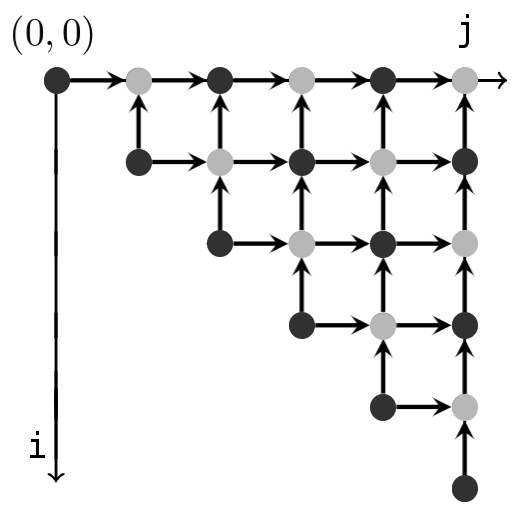
\includegraphics[scale=0.5]{tabulation_01.png}

    \caption{Dependency graph}
    \label{fig:tabulation_01}
\end{figure}

\textbf{Remark :} In a top-down approach, like the one presented in section \ref{susub:memoization}, computing all entries is not mandatory because the sister always picks the local optimum. Some entries of the cache for some subconfigurations will never have to be computed to get an optimal answer, like shown in table \ref{tab:memoization_02}. However, in a bottom-up approach, we will have to compute all entries to get the scores of the final configuration.

\medskip
This does not change the algorithmic complexity which will still be in $O(n^2)$, however it could potentially affect run time. It is a trade-off between getting rid of the recursion overhead and dramatically reducing space complexity (which will be in $O(n)$ for the optimized bottom-up approach), and computing some unnecessary configurations.

\newpage

\ezskip
To get this bottom-up solution to work, we consider the bottom diagonal and move all the way up to the global configuration.
The first diagonal is initialized easily, with :

\begin{equation}
cache[i][i] = (CARDS[i], 0), \ i \in [\![0,\ n-1]\!] 
\end{equation}

We then move up, computing the next stage using the recurrence formula, as described in figure \ref{fig:tabulation_02}. To know whether or not each diagonal corresponds to the first player or the second player picking a card (gray and black colors in the diagram), we just compute the following modulo of the $j$ index of the current diagonal :

\begin{equation}
(j + n) \equiv_{2} 1 \implies sisterFirst_{diag_j} = sisterFirst_{(0,\ n-1)}
\end{equation}
\begin{equation}
(j + n) \equiv_{2} 0 \implies sisterFirst_{diag_j} = \neg \ sisterFirst_{(0,\ n-1)}
\end{equation}

\begin{figure}[H]
    \centering
    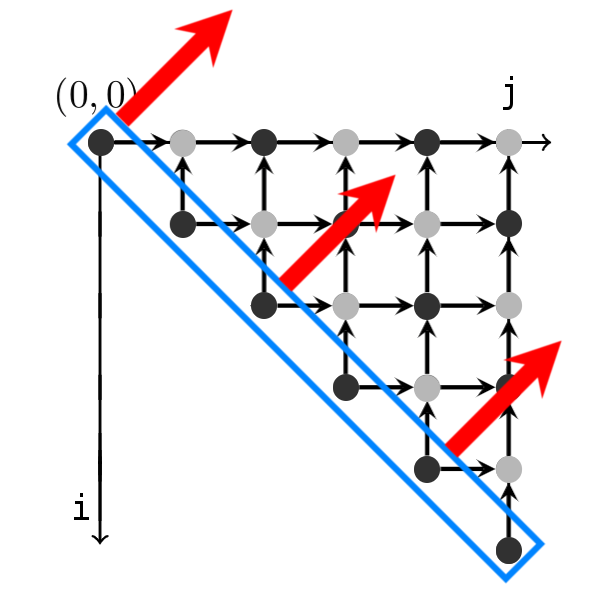
\includegraphics[scale=0.5]{tabulation_02.png}

    \caption{Following the diagonal}
    \label{fig:tabulation_02}
\end{figure}

\noindent
Below is the Python implementation of the bottom-up version of the program :

\begin{minted}[frame=leftline]{Python}
cache = [[0]*LEN_CARDS for _ in range(LEN_CARDS)]
# Finding which player is first on diagonal {diag_index}
def isSisterFirst(diag_index, sisterFirst):
    if ((diag_index + LEN_CARDS)%2 == 1):
        return sisterFirst
    else:
        return not sisterFirst

# Updating a cell value on a diagonal
def updateCell(coord, sisterFirst):
    i,j = coord
    if (sisterFirst):
        # Sister takes the local optimum
        if (CARDS[i] > CARDS[j]):
            firstScore  = CARDS[i] + cache[i+1][j][1]
            secondScore = cache[i+1][j][0]
        else:
            firstScore  = CARDS[j] + cache[i][j-1][1]
            secondScore = cache[i][j-1][0]
    else:
        # Strategist takes the global optimum
        if (CARDS[i] + cache[i+1][j][1] > CARDS[j] + cache[i][j-1][1]):
            firstScore = CARDS[i] + cache[i+1][j][1]
            secondScore = cache[i+1][j][0]
        else:
            firstScore = CARDS[j] + cache[i][j-1][1]
            secondScore = cache[i][j-1][0]
    
    cache[i][j] = (firstScore, secondScore)

def getScores(i, j, sisterFirst):
    if (i==j): return (CARDS[i], 0)

    # Initializing the main diagonal
    for k in range(LEN_CARDS):
        cache[k][k] = (CARDS[k], 0)

    # Computing all cache values diagonal by diagonal
    for diag_index in range(1, LEN_CARDS):
        sisterFirstDiag = isSisterFirst(diag_index, sisterFirst)

        # Updating all cells in the diagonal
        it_coord = [0, diag_index]
        for _ in range(LEN_CARDS - diag_index):
            updateCell(it_coord, sisterFirstDiag)
            it_coord = [x+1 for x in it_coord]

    return cache[0][LEN_CARDS-1]
\end{minted}

No more recursive calls are necessary to obtain the optimal score for the strategist, however we now need to compute every cache value.
As an example, in table \ref{tab:tabulation_03} is the cache obtained when executing this new bottom-up function on the configuration of the aformentioned figure \ref{fig:memoization_01} (as a reminder, table \ref{tab:memoization_02} was the final cache using the top-bottom solution).

\ezskip
This new version of the function returns exactly the same optimal scores and intermediate scores for subconfigurations, however it makes a lot more computations than the top-bottom version. The complexity however still remains the same, and we got rid of the recursion overhead.

\begin{table}[H]
\centering
\begin{TAB}(e,1cm,1cm){|c:c:c:c:c:c:c:c:c:c|}{|c:c:c:c:c:c:c:c:c:c|}
\hline
(14, 0)   &(14, 6)   &(20, 9)   &(23, 13)  &(26, 13)  &(27, 23)  &(37, 26)  &(39, 29)  &(43, 32)  &(46, 31) \\
0         &(6, 0)    &(9, 6)    &(13, 9)   &(13, 12)  &(23, 13)  &(26, 23)  &(29, 25)  &(32, 29)  &(31, 32) \\
0         &0         &(9, 0)    &(9, 7)    &(12, 7)   &(18, 12)  &(25, 18)  &(25, 23)  &(32, 23)  &(32, 25) \\
0         &0         &0         &(7, 0)    &(7, 3)    &(14, 7)   &(20, 14)  &(23, 16)  &(23, 23)  &(25, 23) \\
0         &0         &0         &0         &(3, 0)    &(11, 3)   &(16, 11)  &(16, 16)  &(23, 16)  &(23, 18) \\
0         &0         &0         &0         &0         &(11, 0)   &(13, 11)  &(16, 13)  &(20, 16)  &(18, 20) \\
0         &0         &0         &0         &0         &0         &(13, 0)   &(13, 5)   &(18, 7)   &(20, 7)  \\
0         &0         &0         &0         &0         &0         &0         &(5, 0)    &(7, 5)    &(7, 7)   \\
0         &0         &0         &0         &0         &0         &0         &0         &(7, 0)    &(7, 2)   \\
0         &0         &0         &0         &0         &0         &0         &0         &0         &(2, 0)   \\
\end{TAB}
\caption{Resulting entries for the memoization cache}
\label{tab:tabulation_03}
\end{table}

\newpage
This solution can be further down optimized in memory to $O(n)$ space complexity by storing only two subsequent diagonals at a time.
In figure \ref{fig:tabulation_04} is an illustration of the two diagonals that will be kept in memory at some given point of our iterative process.

\begin{figure}[H]
    \centering
    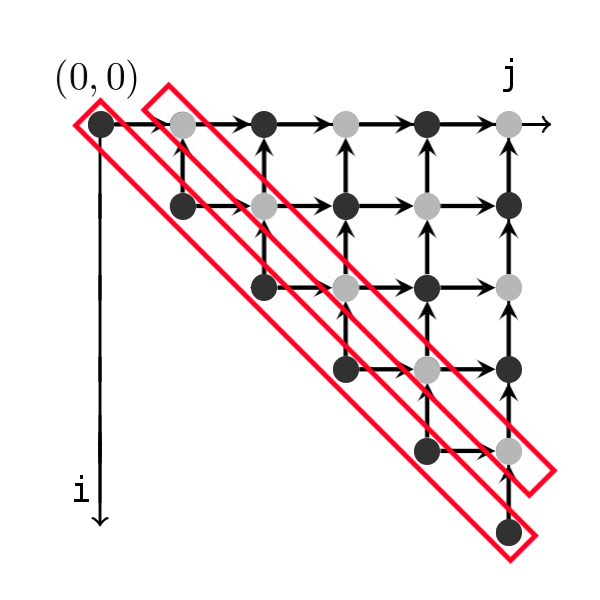
\includegraphics[scale=0.5]{tabulation_04.png}

    \caption{Graph dependency with the two diagonals highlighted}
    \label{fig:tabulation_04}
\end{figure}

Let \texttt{$diag_0$} and \texttt{$diag_1$} be the two arrays of size \texttt{LEN\_CARDS} (or $n$) storing the values highlighted in the figure.
Since \texttt{$diag_1$} is one entry smaller than \texttt{$diag_2$}, we only need to compute $n - 1$ values. In general, for a diagonal of index $j$ we must compute $n - j$ values.

\ezskip
To obtain \texttt{$diag_j[k]$}, we then need to know the values of $diag_{j-1}[k]$ and $diag_{j-1}[k+1]$. In practice, $diag_{j-1}[k]$ will be $cache[i][j-1]$, and $diag_{j-1}[k+1]$ will be $cache[i+1][j]$.

\ezskip
We will then only need to use two arrays of fixed size n to compute the final result, which knocks down our space complexity to $O(2n) = O(n)$.

\medskip
Below is the implementation corresponding to this improvement (function \texttt{isSisterFirst} is as defined earlier) :

\begin{minted}[frame=leftline]{Python}
diags = [[0]*LEN_CARDS for _ in range(2)]

def updateCell(coord, k, sisterFirst, diag_i):
    i,j = coord
    print (k, diag_i)
    if (sisterFirst):
        # Sister takes the local optimum
        if (CARDS[i] > CARDS[j]):
            firstScore  = CARDS[i] + diags[diag_i][k+1][1]
            secondScore = diags[diag_i][k+1][0]
        else:
            firstScore  = CARDS[j] + diags[diag_i][k][1]
            secondScore = diags[diag_i][k][0]
    else:
        # Strategist takes the global optimum
        if (CARDS[i] + diags[diag_i][k+1][1] > CARDS[j] + diags[diag_i][k][1]):
            firstScore = CARDS[i] + diags[diag_i][k+1][1]
            secondScore = diags[diag_i][k+1][0]
        else:
            firstScore = CARDS[j] + diags[diag_i][k][1]
            secondScore = diags[diag_i][j-1][0]

    diags[1-diag_i][k] = (firstScore, secondScore)

def getScores(i, j, sisterFirst):
    if (i==j): return (CARDS[i], 0)

    # Initializing the first diagonal
    for k in range(LEN_CARDS):
        diags[0][k] = (CARDS[k], 0)

    # Computing cache values, starting from the diagonal
    diag_i = 0
    for diag_index in range(1, LEN_CARDS):
        sisterFirstDiag = isSisterFirst(diag_index, sisterFirst)

        # Updating all cells in the diagonal
        it_coord = [0, diag_index]
        for k in range(LEN_CARDS - diag_index):
            updateCell(it_coord, k, sisterFirstDiag, diag_i)
            it_coord = [x+1 for x in it_coord]

        # Flipping the cache entry to use for next diagonal
        diag_i = 1 - diag_i

    return diags[diag_i][0]
\end{minted}
\newpage
Here is a practical example of the resulting cache obtained for the example configuration described earlier in figure \ref{tab:memoization_02} :

\begin{table}[H]
\centering
\begin{TAB}(e,1cm,1cm){|c:c:c:c:c:c:c|}{|c:c:c:c:c:c:c|}
\hline
(18, 13)  &(17, 9)   &(13, 9)   &(16, 9)   &(12, 9)   &(9, 0)    &(4, 0) \\
(25, 10)  &(13, 17)  &(17, 9)   &(16, 12)  &(9, 8)    &(9, 4)    &0      \\
\end{TAB}
\caption{Resulting entries for the diagonals optimized cache}
\label{tab:tabulation_04}
\end{table}

In the first row, in coordinates [0,0] is the final score for both players. Since diagonals don't have to be cleared between computations, old values are simply overwritten and what we see in the cache are mostly values from diagonals computed in previous iterations.

\subsubsection{Tabulation solution complexity}

After replacing the recursive overheads in the memoized version, computing the time complexity gets easier. Indeed, the time-expensive computations are those we do while following the diagonal such as in figure \ref{fig:tabulation_02}. The first diagonal costs $n$ computations, the second one $(n - 1)$ and so on, leading to a total cost of $\sum_{k = 1}^{n} \mathcal{O}(k) = \mathcal{O}(\frac{n(n+1)}{2})$ : the complexity is thus quadratic in $n$.
\ezskip As mentioned earlier, the space complexity is in $\mathcal{O}(n)$.

\subsection{General case}

In the general case, the sister may not always pick the right-most card if she has to choose between two cards of equal cost.
Going down the solution tree, if we get to a point for which we have $CARDS[i] = CARDS[j]$, and the sister is the one playing, we should be exploring both cases. However, in one case the optimal solution exploration might be losing or winning.

\ezskip Thus, to model the best the problem, we should explore both options and compute probabilities of winning for each. As an example, if one subtree leads to a winning optimal solution, and the other leads to a losing one, assuming equiprobability of the sister's choice our program should return a 0.5 probability of winning, instead of a binary answer.

\ezskip
However, we did not have time to implement this version of the solution.

% --------------------------------------------------------------
%                         Conclusion
% --------------------------------------------------------------

\newpage
\section{Conclusion}
%% TODO complete, RESPONSIBLE PERSON: Manuel
Our main goal in this APP is winning a card game regardless of which player starts. We first demonstrated how we could win using a greedy algorithm. However, as winning was not systematic even when we could, we extended our solution to cover all possible solution sets in order to be sure that we can get the best possible score, given the initial configuration of the cards. As this method was not efficient in terms of time complexity, dynamic programming was introduced as the optimum solution for winning (based on assumptions and conditions).

\ezskip In general, the dynamic programming method is one of the few algorithmic techniques that can take problems for which the naive solutions require exponential time and produce polynomial time algorithms. In this APP, dynamic programming was used not only to solve the card game but also to lead us to an optimal game strategy.


\end{document}
